
%(BEGIN_QUESTION)
% Copyright 2014, Tony R. Kuphaldt, released under the Creative Commons Attribution License (v 1.0)
% This means you may do almost anything with this work of mine, so long as you give me proper credit

A set of three 50/51 protective relays is supposed to protect a feeder line supplying power to a number of different industrial loads at 13.8 kV.  After operating for several years without incident an insulator on the feeder line happens to fail, resulting in a phase-to-ground fault lasting long enough to burn down one of the wooden power poles supporting the feeder line.  None of the 50/51 feeder relays trips the circuit breaker automatically as designed.  The fault only cleared when an upstream circuit breaker (closer to the substation) was tripped by its own 51 relay.  Subsequent analysis by system engineers determine that the fault current in the grounded line was high enough that it should have picked up both the 51 and 50 functions in the feeder's protective relay monitoring the faulted phase:

$$\includegraphics[width=15.5cm]{i03120x01.eps}$$

Identify the likelihood of each specified fault in this system, to explain why the breaker failed to trip as it should have to clear the line fault.  Consider each fault one at a time (i.e. no coincidental faults), determining whether or not each fault could independently account for {\it all} observations and symptoms in this circuit.

% No blank lines allowed between lines of an \halign structure!
% I use comments (%) instead, so that TeX doesn't choke.

$$\vbox{\offinterlineskip
\halign{\strut
\vrule \quad\hfil # \ \hfil & 
\vrule \quad\hfil # \ \hfil & 
\vrule \quad\hfil # \ \hfil \vrule \cr
\noalign{\hrule}
%
% First row
{\bf Fault} & {\bf Possible} & {\bf Impossible} \cr
%
\noalign{\hrule}
%
% Another row
125 VDC station power supply dead &  &  \cr
%
\noalign{\hrule}
%
% Another row
52a contact failed open &  &  \cr
%
\noalign{\hrule}
%
% Another row
50-1 coil failed shorted &  &  \cr
%
\noalign{\hrule}
%
% Another row
52TC coil failed open &  &  \cr
%
\noalign{\hrule}
%
% Another row
CT ground connection failed open &  &  \cr
%
\noalign{\hrule}
} % End of \halign 
}$$ % End of \vbox

\underbar{file i03120}
%(END_QUESTION)





%(BEGIN_ANSWER)

% No blank lines allowed between lines of an \halign structure!
% I use comments (%) instead, so that TeX doesn't choke.

$$\vbox{\offinterlineskip
\halign{\strut
\vrule \quad\hfil # \ \hfil & 
\vrule \quad\hfil # \ \hfil & 
\vrule \quad\hfil # \ \hfil \vrule \cr
\noalign{\hrule}
%
% First row
{\bf Fault} & {\bf Possible} & {\bf Impossible} \cr
%
\noalign{\hrule}
%
% Another row
125 VDC station power supply dead & $\surd$ &  \cr
%
\noalign{\hrule}
%
% Another row
52a contact failed open & $\surd$ &  \cr
%
\noalign{\hrule}
%
% Another row
50-1 coil failed shorted &  & $\surd$ \cr
%
\noalign{\hrule}
%
% Another row
52TC coil failed open & $\surd$ &  \cr
%
\noalign{\hrule}
%
% Another row
CT ground connection failed open &  & $\surd$ \cr
%
\noalign{\hrule}
} % End of \halign 
}$$ % End of \vbox

%(END_ANSWER)





%(BEGIN_NOTES)

{\bf This question is intended for exams only and not worksheets!}.

%(END_NOTES)


